\documentclass[onecolumn, draftclsnofoot,10pt, compsoc]{IEEEtran}
\usepackage{graphicx}
\usepackage{url}
\usepackage{setspace}

%Personal imports
%\usepackage{cite}
\newcommand{\subparagraph}{}
\usepackage{titlesec}
\usepackage{hyperref}
\usepackage{xcolor}

%Change link colors
\hypersetup{
    colorlinks=true,
    linkcolor=black,
    citecolor=black,
    filecolor=black,
    urlcolor=black,
}

\usepackage{geometry}
\geometry{textheight=9.5in, textwidth=7in}

\titleclass{\subsubsubsection}{straight}[\subsection]
\titleclass{\subsubsubsubsection}{straight}[\subsection]

\newcounter{subsubsubsection}[subsubsection]
\newcounter{subsubsubsubsection}[subsubsubsection]
\renewcommand\thesubsubsubsection{\thesubsubsection.\arabic{subsubsubsection}}
\renewcommand\thesubsubsubsubsection{\thesubsubsubsection.\arabic{subsubsubsubsection}}
\renewcommand\theparagraph{\thesubsubsubsection.\arabic{paragraph}} % optional; useful if paragraphs are to be numbered

\titleformat{\subsubsubsection}
  {\normalfont\normalsize\bfseries}{\thesubsubsubsection}{1em}{}
\titlespacing*{\subsubsubsection}
{0pt}{3.25ex plus 1ex minus .2ex}{1.5ex plus .2ex}
\titleformat{\subsubsubsubsection}
  {\normalfont\normalsize\bfseries}{\thesubsubsubsubsection}{1em}{}
\titlespacing*{\subsubsubsubsection}
{0pt}{3.25ex plus 1ex minus .2ex}{1.5ex plus .2ex}


\makeatletter
\renewcommand\paragraph{\@startsection{paragraph}{5}{\z@}%
  {3.25ex \@plus1ex \@minus.2ex}%
  {-1em}%
  {\normalfont\normalsize\bfseries}}
\renewcommand\subparagraph{\@startsection{subparagraph}{6}{\parindent}%
  {3.25ex \@plus1ex \@minus .2ex}%
  {-1em}%
  {\normalfont\normalsize\bfseries}}
\def\toclevel@subsubsubsection{4}
\def\toclevel@subsubsubsubsection{5}
\def\toclevel@paragraph{6}
\def\toclevel@paragraph{7}
\def\l@subsubsubsection{\@dottedtocline{4}{11em}{5em}}
\def\l@subsubsubsubsection{\@dottedtocline{5}{16em}{6em}}
\def\l@paragraph{\@dottedtocline{5}{10em}{5em}}
\def\l@subparagraph{\@dottedtocline{6}{14em}{6em}}
\makeatother

\setcounter{secnumdepth}{5}
\setcounter{tocdepth}{5}


% 1. Fill in these details
\def \CapstoneTeamName{		Group}
\def \CapstoneTeamNumber{		35}
\def \GroupMemberOne{			Christopher Carlsen}
\def \GroupMemberTwo{			Yizheng Wang}
\def \GroupMemberThree{			Peter Dorich}
\def \CapstoneProjectName{		Develop an Internet of Things Irrigation Valve}
\def \CapstoneSponsorCompany{	 	OSU \textbar\hspace{.05in} Openly Published Environmental Sensing (OPEnS) Lab}
\def \CapstoneSponsorPerson{		Chet Udell}

% 2. Uncomment the appropriate line below so that the document type works
\def \DocType{		%Problem Statement
	Requirements Document
	%Technology Review
	%Design Document
	%Progress Report
}

\newcommand{\NameSigPair}[1]{\par
	\makebox[2.75in][r]{#1} \hfil 	\makebox[3.25in]{\makebox[2.25in]{\hrulefill} \hfill		\makebox[.75in]{\hrulefill}}
	\par\vspace{-12pt} \textit{\tiny\noindent
		\makebox[2.75in]{} \hfil		\makebox[3.25in]{\makebox[2.25in][r]{Signature} \hfill	\makebox[.75in][r]{Date}}}}
% 3. If the document is not to be signed, uncomment the RENEWcommand below
%\renewcommand{\NameSigPair}[1]{#1}

%%%%%%%%%%%%%%%%%%%%%%%%%%%%%%%%%%%%%%%
\begin{document}
	\begin{titlepage}
		\pagenumbering{gobble}
		\begin{singlespace}
			
\includegraphics[height=4cm]{coe_v_spot1}
			\hfill 
			% 4. If you have a logo, use this include graphics command to put it on the coversheet.
			%\includegraphics[height=4cm]{CompanyLogo}   
			\par\vspace{.2in}
			\centering
			\scshape{
				\huge CS461 Capstone \DocType \par
				{\large\today - Fall Term}\par
				\vspace{.5in}
				\textbf{\Huge\CapstoneProjectName}\par
				\vfill
				{\large Prepared for}\par
				\Huge \CapstoneSponsorCompany\par
				\vspace{10pt}
				{\Large\NameSigPair{\CapstoneSponsorPerson}\par}
				{\large Prepared by }\par
				Group\CapstoneTeamNumber\par
				% 5. comment out the line below this one if you do not wish to name your team
				%\CapstoneTeamName\par 
				\vspace{5pt}
				{\Large
					\NameSigPair{\GroupMemberOne}\par
					\NameSigPair{\GroupMemberTwo}\par
					\NameSigPair{\GroupMemberThree}\par
				}
				\vspace{20pt}
			}
			\begin{abstract}
				% 6. Fill in your abstract   --- TODO 
				This document is the Requirements Specification that will be used to detail the objectives of the Internet of Things Irrigation Valve project.
				It will contain a more specific look at what completion goals for this project are and what a user of the this project's product should reasonably expect.
			\end{abstract}     
		\end{singlespace}
	\end{titlepage}
	\newpage
	\pagenumbering{arabic}
	\tableofcontents
	% 7. uncomment this (if applicable). Consider adding a page break.
	%\listoffigures
	%\listoftables
	\clearpage
	
	% 8. now you write!
	\section{Introduction}
	\subsection{Purpose}
	This requirements specification (RS) document serves to more concretely establish the desired end goals of the Irrigation Valve project.
	Its intended usage is for the Irrigation Valve team and their client, Chet Udell, as well as any third party groups with whom may become involved over the course of the project. 
	\subsection{Scope}
	There will be three overall products of this project, defined a follows -\vspace{-.1in}
	\subsubsection{Soil Moisture Sensor/Valve Control}
	The soil moisture sensor's primary job will be to read moisture data from a pre-existing piece of hardware.
	Upon reading this data, it will send it to a designated data-collection hub.
	This device will also embody the "physical" aspect of this project, as it will be the device that engages or disengages an attached valve.
	\subsubsection{Centralized Data Hub/Command Relay}
	This device will be created to facilitate the transfer of data to and from the valve and web application. This hub will connect to the world wide web via Ethernet shield.
    This Ethernet shield allows our hardware devices to read and write to an SD card for data transfer, as well as access Ethernet libraries. 
	The hub will transmit soil moisture data from the valve to the web application for authorized viewing.
    In turn, the hub will also transmit the conditionals for valve control. 
	\subsubsection{Web-based User Interface/Data Tracker}
	Serving as the "face" of the project, this will be the actual interface with which this system's users will interact.
	The user will use this system to view recorded moisture data from various sensors, as well as use it to make decisions on when and where water is most needed in their field.
	This system will take user input and send it to desired watering schedules (via the relay hub) to the individual sensor/valve-control devices in the desired watering areas.
	\subsection{Definitions, acronyms and abbreviations}
	For purposes of brevity, some abbreviations may be used through out this document as follows:
	\begin{itemize}
		\item{[Sensor/soil sensor/moisture sensor] - Will be used in reference to the "Soil Moisture Sensor/Valve Control" device and its related parts.}
		\item{[Data hub/hub/relay] - Will be used in reference to the "Information Communication Relay/Command" device and its related parts.}
        
        \item{[Internet of Things, IoT] - Will be used in reference to a system of wireless devices that can connect to the Internet, called the Internet of things.}
       	\item{[VWC, Volumetric Water Content] - Will be used as a reference to the ratio of water volume to soil volume. This numerical measure is the basic unit for our soil moisture sensors.}
		\item{[UI/Interface/database/tracker] - Will be used in reference to the "Web-based User Interface/Data Tracker" device and its related parts.}
        \item{[LoRa/Long Range radio] - Will be used in reference to a wireless communication standard known as Long Range radio (LoRa radio is a specific type of "long range radio").}
	\end{itemize}
	\subsection{References}
	See Appendix A
	\subsection{Overview}
	%TODO
    The rest of this document outlines what our project is, and goes over functional requirements.
    Section 2, Overall desription, will go over the high level view of the project, and even cover some design constraints. 
    Section 3 will cover the specific requirements of our project. 
    This includes everything from hardware and software packages, to the purpose of each subsection of the project. 
    
    
	\section{Overall description}
	\subsection{Product perspective}
	This projects final product, a soil-moisture data tracking and informed irrigation valve control system, will stand as an individual product composed of three parts.
	The product, however, will be included under a blanket project group known as Project Loom.
	It will not be reliant on other Project Loom products for any functionality, but may potentially be considered as a competent part of an overall package delivered by Project Loom.
	
	%TODO - FILL OUT remainder of this section with information regarding
	% a) System interfaces;
	% b) User interfaces;
	% c) Hardware interfaces;
	% d) Software interfaces;
	% e) Communications interfaces;
	% f) Memory;
	% g) Operations;
	% h) Site adaptation requirements;
	% (See section 5.2.1 for more information)
	
	\subsection{User characteristics}
	The user for our project can have a very minimal level of education and technical experience.
    It is, however, assumed that the user knows how to water their land, and that they understand what they are using our product for. 
    The user will not interact with the wireless hub, or the valve and sensors. 
    The user will only be expected to interact with the web client. 
    Later in the document, there are multiple specific requirements concerning how the user interface is layed out, in order to ensure that our system is usable. 
    Our user interface mostly consists of drop-down menus and input boxes for integer values, making it very intuitive. 
    \subsection{Constraints}
	The following are design constraints for the project, regarding the software and hardware components.
	These constraints are hardware and software that the client has specifically requested be used in the project.
	These requests were made because the technologies and hardware are already being used in the organization, and are needed in order to maintain compatibility and uniformity. 
	\begin{itemize}
		\item{32u4 RFM95 LORA Radio with 915 MHz processors (sensors and hub)}
		\item{Ethernet Shield (hub)}
		\item{Arduino IDE (sensors and hub)}
		\item{MQTT (hub and user interface)}
	\end{itemize}
	\subsection{Assumptions and dependencies}
    Since our design constraints are almost entirely based off of using technology that is compatible with current OPEnS software, the assumptions and dependencies are related to interactions between them. 
    For example, it is worth noting that if upon execution of the project, we learn that MQTT is incompatible for a specific action, we will have to look for a new solution. 
    A system with as many different moving parts has a decent potential to run into these issues, however, the research into our required hardware and software proves that our system is well designed and everything should be compatible. 

%Section 3 from here ---
\section{Specific requirements}
	\subsection{External interface requirements}
    	\subsubsection{User interfaces}
        The project helps users to adjust the behavior of valve through a web client. 
        It is implemented in two parts. 
        The first part is that the user can view the status of all fields on one page. Those status' include the unique ID of each sensor, VWC(Volumetric Water Content) which shows the condition of soil moisture, on/off of the valve, current mode to control the valve, and date and the time that data comes in. 
        The user may view the detailed setting of the current mode by clicking the button of the “current mode” cell.
        The user can view the log, which includes an error message and past operations (this should include mode change and setting change for mode) by clicking the log button on navigation menu under the title of the page.
        *(There will be a single page that contains brief guide about this web client.)
        There will be a single page about the whole project. 
        This includes the people that developed the project, and the address of source code.
        There is also an introduction of this project as well.
        The second part is for the user to change the behavior of the valve.
        There are three modes for the user to control the valve.
        The user can change the mode of each valve by clicking the button beside the "current mode" cell. 
        After that, the button will expand into an input field for the user to change the settings.
        The three modes need different input. 
        In gerneral, there are two inputs needed. 
        The first is the duration for the valve being open, which includes a start time and end time.
        The start date decides the time for valve to turn on, and end date decides the time for valve to turn off.
        The user can enter the dates by clicking the schedule module (or enter them in input box).
        The second is the VWC value, which should be number range from 0 to 100 and also includes two values.
        When VWC is lower than the lower bound, the valve will turn on.
        When the VWC value is higher than the higher bound, the valve will turn off.
        The user may enter the VWC values into two separate input boxes.
        After entering all the inputs, the user can click apply button to apply the changes. The web client will check the input.
        \subsubsection{Hardware interfaces}
        Hardware interfaces for this project will be limited to the sensor and hub devices.
        The sensor device will interact with other hardware in three separate ways.
        The first and most crucial hardware interaction of the project is the interaction betwen
        interaction for the sensor device will be to read soil moisture data from the Decagon soil moisture sensing device.
        This interaction will occur by attaching the moisture device directly to an Adafruit Feather via soldering.
        The 
        \subsubsection{Software interfaces}
        In order to set up our system, we will utilize multiple pieces of software.      
        The first being MQTT, which stands for machine-to-machine Internet of Things connectivity protocol.
        This was created as a lightweight messaging protocol with a small amount of code.   
        This software is best used for mobile uses because if its efficient structure.       
        MQTT, for our purposes, will be used as our connection protocol between our hub and the world wide web. 
        In addition, IFTTT will also be used in conjunction with MQTT. 
        IFTTT stands for if this then that, and it is used as a conditional protocol between existing services such as Google and Facebook.
        IFTTT will specifically be used to control what happens to our system based on what the user inputs on the web application. 
        The Arduino integrated development environment will be used to program the Adafruit micro-controllers.
        Arduino is an open source software package that is used across a wide variety of control boards.
        Our Adafruit boards are completely compatible with Arduino package, making development possible. 
        Another software library we will utilize is the SDI-12 Arduino package.
        This software allows us to connect our Arduino-based micro-controller to our SDI-12 moisture sensors. 
        SDI-12 is an existing communication protocol for environmental sensors. 
        This software package will allow us to receive the electrical data from the SDI-12 enabled moisture sensor.
        This package is required to make our sensors compatible with the Arduino libraries. 
        
        \subsubsection{Communication interfaces} Our system is aimed at the flow of information from the environment to the user, so naturally, communication interfaces are extremely important.
        Introduced in the software interfaces, MQTT will be used as our own communication protocol between our boards. 
        Communication between devices will be done with small messages indicating actions. 
        The messages are dumped into MQTT, where they are visible to the hub and the web application. 
        Then, the hub and the application can take action based on the messages present. 
        MQTT and IFTTT will not work with each other at all, but rather in conjunction with each other.
        MQTT is a communications protocol that will allow us to make a conditional structure of our very own from scratch, while IFTT works to allows us to work with established programs, like Google. 
       In this section, it should be noted that the hub and the web client will not explicitly be connected, and use MQTT and the adafruit in order to exchange information. 
    \subsection{System features}
      \subsubsection{Soil Moisture Sensor/Valve Control}
      \begin{itemize}
          \item{As a user, I want the sensor device to that take moisture data samples every 15 minutes.}
          \item{As a user, I want the irrigation valve turned on or off, based on a set of conditionals triggers that I set.}
          \item{As a user, I want a fail-safe/contingency set of instructions that the device will fall back on should it lose contact with the hub device or Internet.}
      \end{itemize}

      \subsubsection{Information Communication Relay/Command}
			\subsubsubsection{Purpose} 
 	  The purpose of this system feature is to transmit data.
      By the inherent nature of our system design, data cannot be transmitted directly between the web application and the valve due to constraints on the hardware.
      In addition, the overhead associated with transmitting so much information is much too large for one Adafruit 32u4. 
      The hub will allow us to process the information and make sense of it before relay through an ethernet shield to be read by the web client. 
      As with our other project deliverables, this section is also aimed at proof of concept, or minimal viable products.
    		\subsubsubsection{Stimulus/Response}
      The hub will accept a wide variety of input and output.
      It will communicate with both the web application and the valve, packaging information as it is being sent.
      There are a few cases in which different data is sent out.\par 
      
      In one case, the user will transmit information through the hub to the valve. 
      This information will include parameters for operation which includes but is not limited to the date, duration of valve operation, and a unique I.D.
      In another case, the valve will be transmitting soil moisture data and valve states through the hub back to the web application. 
      In all cases, the hub will package the relevant data up for transport. 
      \subsubsubsection{Associated Functional Requirements}
     The following are functional requirements for the hub section of the project. 
     These are organized in order of scheduled completion, and the previous must be accomplished before moving forward in most cases.  \subsubsubsubsection{Functional Requirement 1}
          \begin{itemize}
              \item{System must communicate to and from the hub to a computer using Long Range Radio Frequency. 
              This is measurable by testing with a text file, and checking for data integrity.}
  \subsubsubsubsection{Functional Requirement 2}
              \item{The hub needs to be able to send and receive information from both the valve and the web application. 
              A simple text file or data file should arrive safely to and from the valve device and the web application.}
             \subsubsubsubsection{Functional Requirement 3}
             \item{The hub must be able to send the valve a start time and a duration for operation, which can be measured by assurance that the valve opens and closes when specified.} 
             \subsubsubsubsection{Functional Requirement 4} \item{(\textbf{Stretch Goal}) The hub must be able to connect and control two different valves independently, using a unique I.D. Success can be measured by witnessing successful, independent operations on two different valves.}
          \subsubsubsubsection{Functional Requirement 5}
             \item{The hub and the user must be able to specify three different modes on which the valve can operate.
             1: The valve opens and closes based on soil moisture data alone.
             2: The valve opens and closes based on the time of day, in real time.
             Real time for this project is defined as a value within 15 seconds of real time.
             3: The valve opens and closes based on both time of day and soil moisture data.} 
             \subsubsubsubsection{Functional Requirement 6}
             				\item{(\textbf{Stretch Goal}) In addition to the 3 modes listed above, a 4th mode is entirely manual, in which the user will control all aspects of valve function.}
            \subsubsubsubsection{Functional Requirement 7} 
			\item{The hub should receive the volumetric water content (VWC) from the valve and the soil moisture sensors.
            The VWC is the parameter for the moisture content in the soil, and is the main piece if data we are trying to collect from the sensors.
            The data should safely arrive to the computer from the sensors, through the hub.}
            \subsubsubsubsection{Functional Requirement 8}
            
            \item{If the hub goes down due to an unexpected issue or connection loss, the valve must turn to an "off" state, to not let water escape.
            This is a high priority functional requirement.}
          
          \end{itemize}

      \subsubsection{Web-based User Interface/Data Tracker}
      \begin{itemize}
      	\subsubsubsection{Purpose} 
        \item{The purpose of the web client is to interact with users, which includes displaying the output appropriately, and receive input from users.}
        \subsubsubsection{Stimulus/Response}
        \item{The web client will not directly send or receive data from the hub.
        The hub will upload the data to the Adafruit first, then the web client will pull the data from Adafruit within a certain period. Once a user applies the input he entered, the web client should record those changes and check if anything needs to be sent to hub.}  
        \subsubsubsection{Associated Functional Requirements} 
      	  \subsubsubsubsection{Functional Requirement 1}
          \item{The web client needs to be able to send and receive data from hub. 
          A text file should arrive safely to and from the hub.}
          \subsubsubsubsection{Functional Requirement 2}
          \item{The web client should be able to change the mode of valve according to the input from the user.
          This can be checked by setting some extreme value.
          For example, turn on the valve when VWC is lower than 100, or turn off the valve when VWC is higher than 0.}
          \subsubsubsubsection{Functional Requirement 3}
          \item{The web client should be able to list the status of all sensors correctly and appropriately.
          This can be checked by comparing the data that is directly read from the sensors and the displayed information. }
          \subsubsubsubsection{Functional Requirement 4}
          \item{If the hub or the valve shut down, the web client should be able to send warning to user by email or some other approaches. Can be checked by powering off the hub.}
      \end{itemize}   
      
\subsection{Performance Requirements}
This project, as has been noted in this document, is a proof-of-concept, minimal viable product design.
As such, there are not many performance requirements in terms of system efficiently.
That being said, this does not allow us to make our system terribly inefficient. 
Thinking about our application, system decisions based on soil data must execute quickly, and cant take hours to process. 
In order to ensure we have some degree of accuracy, we will make our system run on plus or minus 15 seconds of real time. 
This allows a minimal amount of room, while still maintaining an excellent degree of accuracy. 
	%Section{Gantt Chart}
	\noindent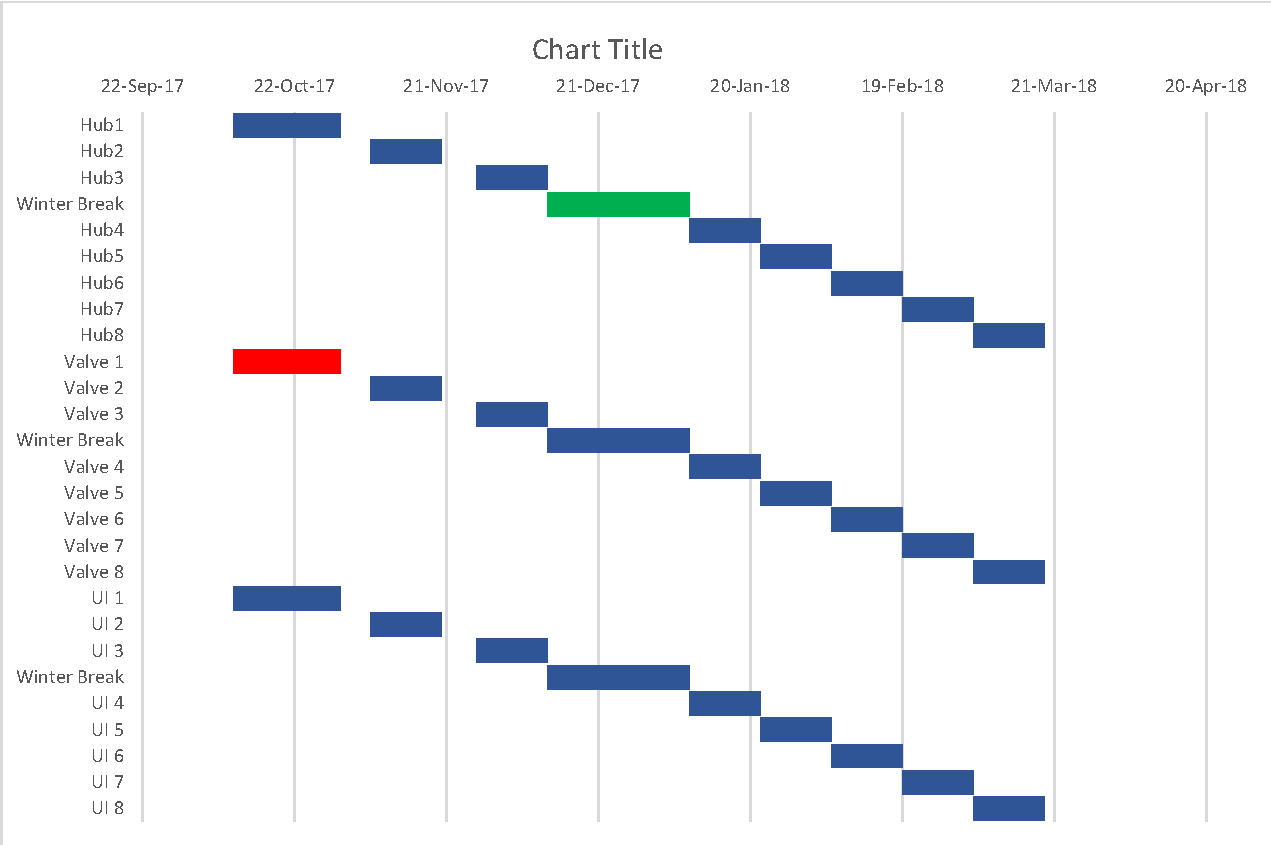
\includegraphics[width=\linewidth]{chart_cropped}
	
	\newpage
	\section{Appendix A - Bibliography}
	\nocite{*} %TODO - Remove this if citing things.
	\bibliographystyle{IEEEtran}
	\bibliography{references}
	
\end{document}